\documentclass[tikz,border=6pt]{standalone}
\usepackage{pgfplots}
\usepackage{amsmath}
\usetikzlibrary{
  arrows.meta,
  backgrounds,
  calc,
  fit,
  matrix,
  positioning,
  shapes.callouts,
  shapes.geometric,
  shapes.misc
}
\pgfplotsset{compat=1.18}

\definecolor{archInk}{HTML}{1F2933}
\definecolor{archBlue}{HTML}{0B4F6C}
\definecolor{archTeal}{HTML}{1B998B}
\definecolor{archGold}{HTML}{D98E04}
\definecolor{archRose}{HTML}{C44536}
\definecolor{archSage}{HTML}{7A9E7E}
\definecolor{archMist}{HTML}{E9F1F7}
\definecolor{archSand}{HTML}{F4F1DE}
\definecolor{archSlate}{HTML}{5C677D}
\definecolor{archStone}{HTML}{C8D0D9}

\tikzset{
  every node/.style={font=\sffamily\small, text=archInk},
  axis label/.style={font=\sffamily\footnotesize, text=archInk},
  panel/.style={
    rounded corners=6pt,
    draw=archSlate,
    line width=0.9pt,
    fill=white
  },
  stage/.style={
    panel,
    fill=archMist,
    minimum height=1.5cm,
    inner sep=7pt,
    align=left
  },
  note/.style={
    panel,
    fill=archSand,
    inner sep=7pt,
    align=left
  },
  verdict/.style={
    panel,
    fill=archTeal!12,
    inner sep=7pt,
    align=left
  },
  kill/.style={
    panel,
    fill=archRose!12,
    draw=archRose,
    inner sep=7pt,
    align=left
  },
  muted/.style={
    panel,
    fill=archStone!20,
    draw=archStone!80!archInk,
    inner sep=6pt,
    align=left
  },
  link/.style={
    -{Latex[length=3mm,width=1.7mm]},
    line width=1.0pt,
    draw=archBlue
  },
  dashedlink/.style={
    -{Latex[length=3mm,width=1.7mm]},
    line width=1.0pt,
    draw=archRose,
    dashed
  }
}

\pgfplotsset{
  every axis/.append style={
    line width=0.9pt,
    tick style={draw=archSlate},
    axis line style={draw=archSlate},
    label style={font=\sffamily\small, text=archInk},
    ticklabel style={font=\sffamily\footnotesize, text=archInk},
    legend style={
      draw=none,
      fill=white,
      font=\sffamily\footnotesize,
      text=archInk
    },
    title style={font=\sffamily\small\bfseries, text=archInk},
    grid style={draw=archStone},
    major grid style={draw=archStone},
    minor grid style={draw=archStone!70}
  }
}

\begin{document}
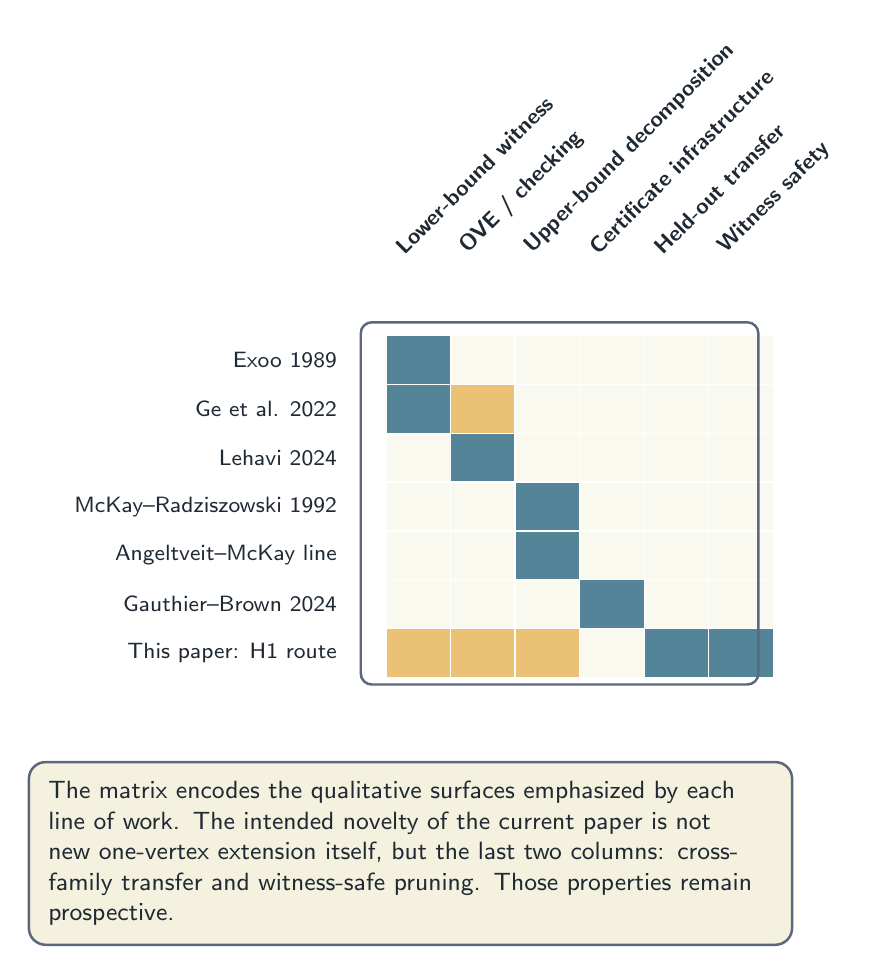
\begin{tikzpicture}[x=1cm,y=1cm]
  \def\cellw{0.82}
  \def\cellh{0.62}
  \def\leftpad{4.6}

  \foreach \i/\lab in {
    0/{Lower-bound witness},
    1/{OVE / checking},
    2/{Upper-bound decomposition},
    3/{Certificate infrastructure},
    4/{Held-out transfer},
    5/{Witness safety}
  }{
    \node[rotate=45, anchor=west, font=\sffamily\footnotesize\bfseries, text=archInk]
      at ({\leftpad + \i*\cellw + 0.08}, 4.85) {\lab};
  }

  \foreach \j/\row/\a/\b/\c/\d/\e/\f in {
    0/{Exoo 1989}/2/0/0/0/0/0,
    1/{Ge et al. 2022}/2/1/0/0/0/0,
    2/{Lehavi 2024}/0/2/0/0/0/0,
    3/{McKay--Radziszowski 1992}/0/0/2/0/0/0,
    4/{Angeltveit--McKay line}/0/0/2/0/0/0,
    5/{Gauthier--Brown 2024}/0/0/0/2/0/0,
    6/{This paper: H1 route}/1/1/1/0/2/2
  }{
    \node[anchor=east, font=\sffamily\footnotesize] at (4.1,{3.54-\j*\cellh}) {\row};
    \foreach \k/\val in {0/\a,1/\b,2/\c,3/\d,4/\e,5/\f}{
      \ifnum\val=0
        \def\fillc{archSand!45}
      \fi
      \ifnum\val=1
        \def\fillc{archGold!55}
      \fi
      \ifnum\val=2
        \def\fillc{archBlue!70}
      \fi
      \draw[draw=white, line width=0.5pt, fill=\fillc]
        ({\leftpad+\k*\cellw},{3.85-\j*\cellh}) rectangle ++(\cellw,-\cellh);
    }
  }

  \draw[archSlate, line width=0.9pt, rounded corners=4pt]
    (4.28,4.02) rectangle (9.33,-0.58);

  \node[note, text width=9.2cm, anchor=north west] at (0.05,-1.55) {
    The matrix encodes the qualitative surfaces emphasized by each line of work. The intended
    novelty of the current paper is not new one-vertex extension itself, but the last two columns:
    cross-family transfer and witness-safe pruning. Those properties remain prospective.
  };
\end{tikzpicture}
\end{document}
